
\documentclass[journal,12pt,twocolumn]{IEEEtran}
\usepackage{tkz-euclide} % loads TikZ and tkz-base
\usepackage{hyperref}
\usepackage{xcolor}
\title{AI1110 Software Project Report}
\author{Pooja Mane\\ (CS22BTECH11035)}
\date{\today}

\begin{document}

\maketitle

\section{Introduction}
This report presents an analysis of the code implementing the Pygame library in a Python script. The code aims to create a simple audio player that plays a shuffled playlist of audio files. 

\section{Implementation}
The project is organized into classes and functions to handle different aspects of the music player. The code is structured as follows:

\begin{itemize}
\item Importing necessary libraries and initializing Pygame.
\item Importing Required Modules: The code starts by importing the necessary modules, including os and random, to handle file operations and generate random numbers.
\item Creating the Pygame window and initializing the mixer for audio playback.
\item Event Handling: The code enters a  loop where it continuously listens for Pygame events. 
\item Setting up the initial song list and play stack.
\item Setting up the main loop to handle events and update the screen.
\item Loading and playing the selected song using Pygame's mixer.
\end{itemize}

\subsection{Dependencies}
To run the Music Player, the following dependencies are required:

\begin{itemize}
\item Python 
\item Pygame library
\item NumPy library
\end{itemize}

Additionally, the following modules are used:

\begin{itemize}
        \item sys
        \item os
\end{itemize}

\section{Conclusion}
The Music Player project provides a basic music player application with features such as playing audio files, controlling playback, and displaying the currently playing song. It demonstrates the use of Pygame and its audio capabilities in Python programming.

\begin{figure}
    \centering
    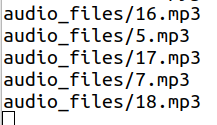
\includegraphics{audio.png}
    \caption{random shuffle}
    \label{fig:my_label}
\end{figure}

\end{document}

